%Material and Methods

In all cases the Pearson's correlation coefficient was used to evaluate and compare the predictive performance the the three methods, PSSM, SVM and ANN

\subsection*{PSSM}
A Position-specific scoring matrix, also called position weight matrix is a commonly used representation of motifs in biological sequences. 
It has one row for each symbol in the alphabet (amino acid, for instance) and one column for each position in the motif.
The weight matrix is constructed using log-odds score

\begin{equation}
W_{ij} = \log{ (\frac{p_{ij}}{q_j}) }
\end{equation}

i being the position in the motif and j the amino acid. $q_j$ is the background frequency for amno acid j. 
The score of a sequence is simply the sum of the position-specific scores for each symbol in the substring.

\begin{equation}
s = \sum_{i}{W_{i}} \\
\end{equation}

where j represents position in the substring, i is the symbol at position j in the substring and $W_{i}$ is the corresponding score in the weight matrix.

PSSM scores can be interpreted as the sum of binding energies for all nucleotides or amino acids aligned with the PSSM and can as such be used to estimate MHC peptide binding affinity.

Sequence weighting can be used to reduce redundancy and emphasize diversity. In the case of MHC peptide binding it is used to compensate for poor or biased sampling of sequence space.
Simply put, the weight on a peptide k at position p is

\begin{equation}
w_{kp} = \frac{1}{r\cdot s}
\end{equation}

where r is the number of different amino acids in the column p, and s is the number of occurence of amino acids a in that column. The weight of the sequence k is then the sum of the weights over all positions

\begin{equation}
w_{k} = \sum_{p}{\frac{1}{r_p \cdot s_p}}
\end{equation}

Pseudo count is used to compensate for few data points and is estimated as

\begin{equation}
g_b = \sum{f_a}{q_{b|a}}
\end{equation}

where $f_a$ is the observed amino acid frequency. The $q_{a|b}$ is the probability of amino acid b given amino acid a and is aquired from a Blosum substitution frequency matrix.
The Blosum substitution matrix, is a
conditional probability matrix of matching amino
acids j given you have amino acid i

\begin{equation}
P(j|i) = \frac{P_ij}{Q_i}
\end{equation}

the matrix is used to for the pseudo count in creation of the PSSM matrix. 

Psuedo counts are important when only limited data is available. With large datasets only the observation should count:

\begin{equation}
p_a = \frac{\alpha \cdot f_a + \beta \cdot g_a}{\alpha + \beta}
\end{equation}

$\alpha$ is the effective number of sequences and $\beta$ is the weight on prior and concerns the size of the data set when pseudo count are taken into account.

The information content of a position in a peptide an indicator of how different its distribution is from a uniform distribution and is calculated using Shannon's discrete entropy law (the sum part of the equation \ref{info})

\begin{equation}
\label{info}
I = \log{ 20 } + \sum_{a}{ p_{a}\log{p_{a}} }
\end{equation}

where $p_a$ is the probability of the symbol a in sequence (for some position in the peptide). The information content is used to estimate which positions in a peptide are more important to the MHC binding than others 
(and to construct so called sequence logos).

\subsection*{SVM}
Support vector machines is a set of supervised learning methods used for classification and regression analysis. 
The standard SVM is non-probabilistic binary linear classifier. 
It constructs a hyperplane where the separation is where there is largest distance to the nearest training data point of any class. 
Nonlinear classification can be achived by  mapping the original space to a higher dimensional feature space and/or select a kernel function to suit the problem. 
The kernel function then plays the role of the dot product in the feature space.

In the linear SVM we want to find the maximum-margin hyperplane that divides the points having (class) $y_{i}$ = 1 from those having $y_i = -1$. Any hyperplane can be written as the set of points \b{x} satisfying

\begin{equation}
\mathbf{w \cdot x} - b = 0
\end{equation}

We want to choose the \b{w} and b to maximize the margin, or distance between the parallel hyperplanes that are as far apart as possible while still separating the data. These hyperplanes can be described by the equations

\begin{equation}
\mathbf{w \cdot x} - b = 1
\end{equation}

and

\begin{equation}
\mathbf{w \cdot x} - b = -1
\end{equation}

The distance between these two hyperplanes is $\frac{2}{||w||}$, so we wan't to minimize $||w||$.
To prevent data points falling into the margin, we add the following constraint:

\begin{equation}
y_i(\mathbf{w \cdot x} - b) \geq 1, for all 1 \leq i \leq n
\end{equation}

where $y_i$ is the class point i belongs to.

Substituting $||w||$ with $\frac{1}{2}||w||^2$ makes this a quadratic optimization problem. 
The solution involves constructing a dual problem where 
a Lagrange multiplier $\alpha_i$ 
is associated with every 
constraint in the primary problem. Mathematically put, find $\alpha_1 \cdots \alpha_n$
such that

\begin{equation}
\mathbf{Q(\alpha)} = \sum_{i=1}^{n}{\alpha_i} - \frac{1}{2}\sum_{i,j}{\alpha_i\alpha_j y_i y_j \mathbf{x_i^T x_j} }
\end{equation}

is maximized knowing $\mathbf{w} = \sum_{i}{ \alpha_i y_i \mathbf{x_i} }$ and $\sum_{i}{\alpha_i y_i} = 0$ and $\alpha_i \geq 0$ for all $\alpha_i$.  
A common method for solving the QP problem is the Sequential Minimal Optimization (SMO) algorithm, 
which breaks the problem down into 2-dimensional sub-problems that may be solved analytically, eliminating the need for a numerical optimization algorithm.
We choose the SMO method for classification in the Weka software.

\subsection*{ANN}
Artificial neural networks are used to model complex relationships between inputs and outputs or to find patterns in data.
Neural networks are non-linear statistical data modeling tools, in most cases an adaptive system that changes its structure based on external or internal information that flows through the network during the learning phase.
The effect on the binding affinity of
having a given amino acid at one
position can be influenced by the
amino acids at other positions in the
peptide. Artificial neural networks are
ideal to take such
correlations into account. Similar to equation \ref{info} a mutual information is defined as

\begin{equation}
\label{mutinfo}
I = \sum_{a,b}{ p_{ab}\log{ \frac{ p_{ab} }{ p_a \cdot p_b } } }
\end{equation}

where $p_{ab}$ is the probability of having amino acids of type a and b in certain positions of the peptide. $p_a$ and $p_b$ are the probabilities of having the corresponding amino acids in the relevant positions in the peptide.
Having sequence correlations demands the classifier to be able to do model a non-linear function (XOR function). Neural network achieve this by adding a hidden layer/neurons.

Associated with every edge of the neural network graph is a weight $w_i$, so the output becomes:

\begin{equation}
o = \sum{x_i \cdot w_i}
\end{equation}

The sigmoid function is used for the output of each neuron:

\begin{equation}
O = \frac{1}{1+\exp{(-o)}}
\end{equation}

The adaptation in the network is achieved by minimizing error by varying the weights. The quadratic error is defined as:

\begin{equation}
E = \frac{1}{2}\sum_{\alpha i}{(O_i^\alpha - T_i^\alpha)^2}
\end{equation}

Then the weights are varied for example with the gradient descent method

\begin{equation}
\Delta w = -\epsilon \frac{\delta E}{\delta w}
\end{equation}

\subsection*{Overfitting}
Overfitting occurs when a statistical model describes random error or noise instead of the underlying relationship.
This can happen when a model is excessively complex, such as having too many parameters relative to the number of observations.
To prevent overfitting a cross-validated training is used. 1/5 of the data is preserved for testing and 4/5 for training. 
The training is stopped when the test performance is optimal. This is done for each of the 5 sections of the data and the result is 5 different sets of network weights/synapses.
All the synapses are then used when evaluating the network.
Optimally one would take one part of the data aside for final evaluation of the network. This part would be used in neither the training nor the testing.
We wanted to have as large sets of peptide data as possible. For the smaller datasets we made a cross-validated training/testing on the whole dataset and then evaluated with testing data using synapses not created with that testing dataset.
As a result the networks for the smaller datasets are possibly slightly overfit (e.g. evaluation data is also in the the training data).
For the larger datasets, we also took 1/5 of the data aside for the evaluation and did a 4-fold cross-validation on the remaining 4 parts.

We mostly used peptide binding data from class-I MHC molecules (A and B types) as they were readily available to us.
To get a better grasp on the the expected quality of the results in the machine learning methods we did evaluate the fraction between binding and non-binding peptides in the dataset for each data {\ref{ftable}}

\begin{table}[th]\scriptsize
\begin{center}
\begin{tabular}{rllrrr}
\hline
 & Allele	&	 binders & non-binders & \% of binders \\
\hline
 & A2402	&	99	&	197	&	50\%	\\
 & A2301	&	49	&	104	&	47\%	\\
 & A0202	&	649	&	1447	&	45\%	\\
 & A0203	&	639	&	1443	&	44\%	\\
 & A6801	&	498	&	1141	&	44\%	\\
 & B4501	&	49	&	114	&	43\%	\\
 & A2902	&	68	&	160	&	43\%	\\
 & B5301	&	106	&	254	&	42\%	\\
 & B1801	&	47	&	118	&	40\%	\\
 & A0201	&	1181	&	3089	&	38\%	\\
 & B4402	&	44	&	119	&	37\%	\\
 & A0206	&	513	&	1437	&	36\%	\\
 & A1101	&	693	&	1985	&	35\%	\\
 & B5101	&	85	&	244	&	35\%	\\
 & B4002	&	39	&	118	&	33\%	\\
 & B5401	&	81	&	255	&	32\%	\\
 & A3002	&	29	&	92	&	32\%	\\
 & B3501	&	211	&	736	&	29\%	\\
 & B4403	&	34	&	119	&	29\%	\\
 & A6802	&	397	&	1434	&	28\%	\\
 & A0301	&	517	&	2094	&	25\%	\\
 & A3101	&	427	&	1869	&	23\%	\\
 & B5701	&	11	&	59	&	19\%	\\
 & B1501	&	179	&	978	&	18\%	\\
 & B0702	&	208	&	1262	&	16\%	\\
 & A3301	&	184	&	1140	&	16\%	\\
 & A3001	&	77	&	669	&	12\%	\\
 & A2403	&	29	&	254	&	11\%	\\
 & B5801	&	104	&	988	&	11\%	\\
 & A6901	&	86	&	833	&	10\%	\\
 & A0101	&	103	&	1157	&	9\%	\\
 & A2601	&	53	&	672	&	8\%	\\
 & B2705	&	56	&	969	&	6\%	\\
 & B4001	&	40	&	1078	&	4\%	\\
 & B0801	&	20	&	708	&	3\%	\\
\hline
\end{tabular}
\caption{Content of bindigs and not bindigs peptides for each allele dataset. The samples are in decreasing order of the percentage of binding peptides.}\label{ftable}
\end{center}
\end{table}

In the PSSM case only the binders are used, so datasets with few of them could give bad results.

\begin{figure*}[ht]
\begin{center}
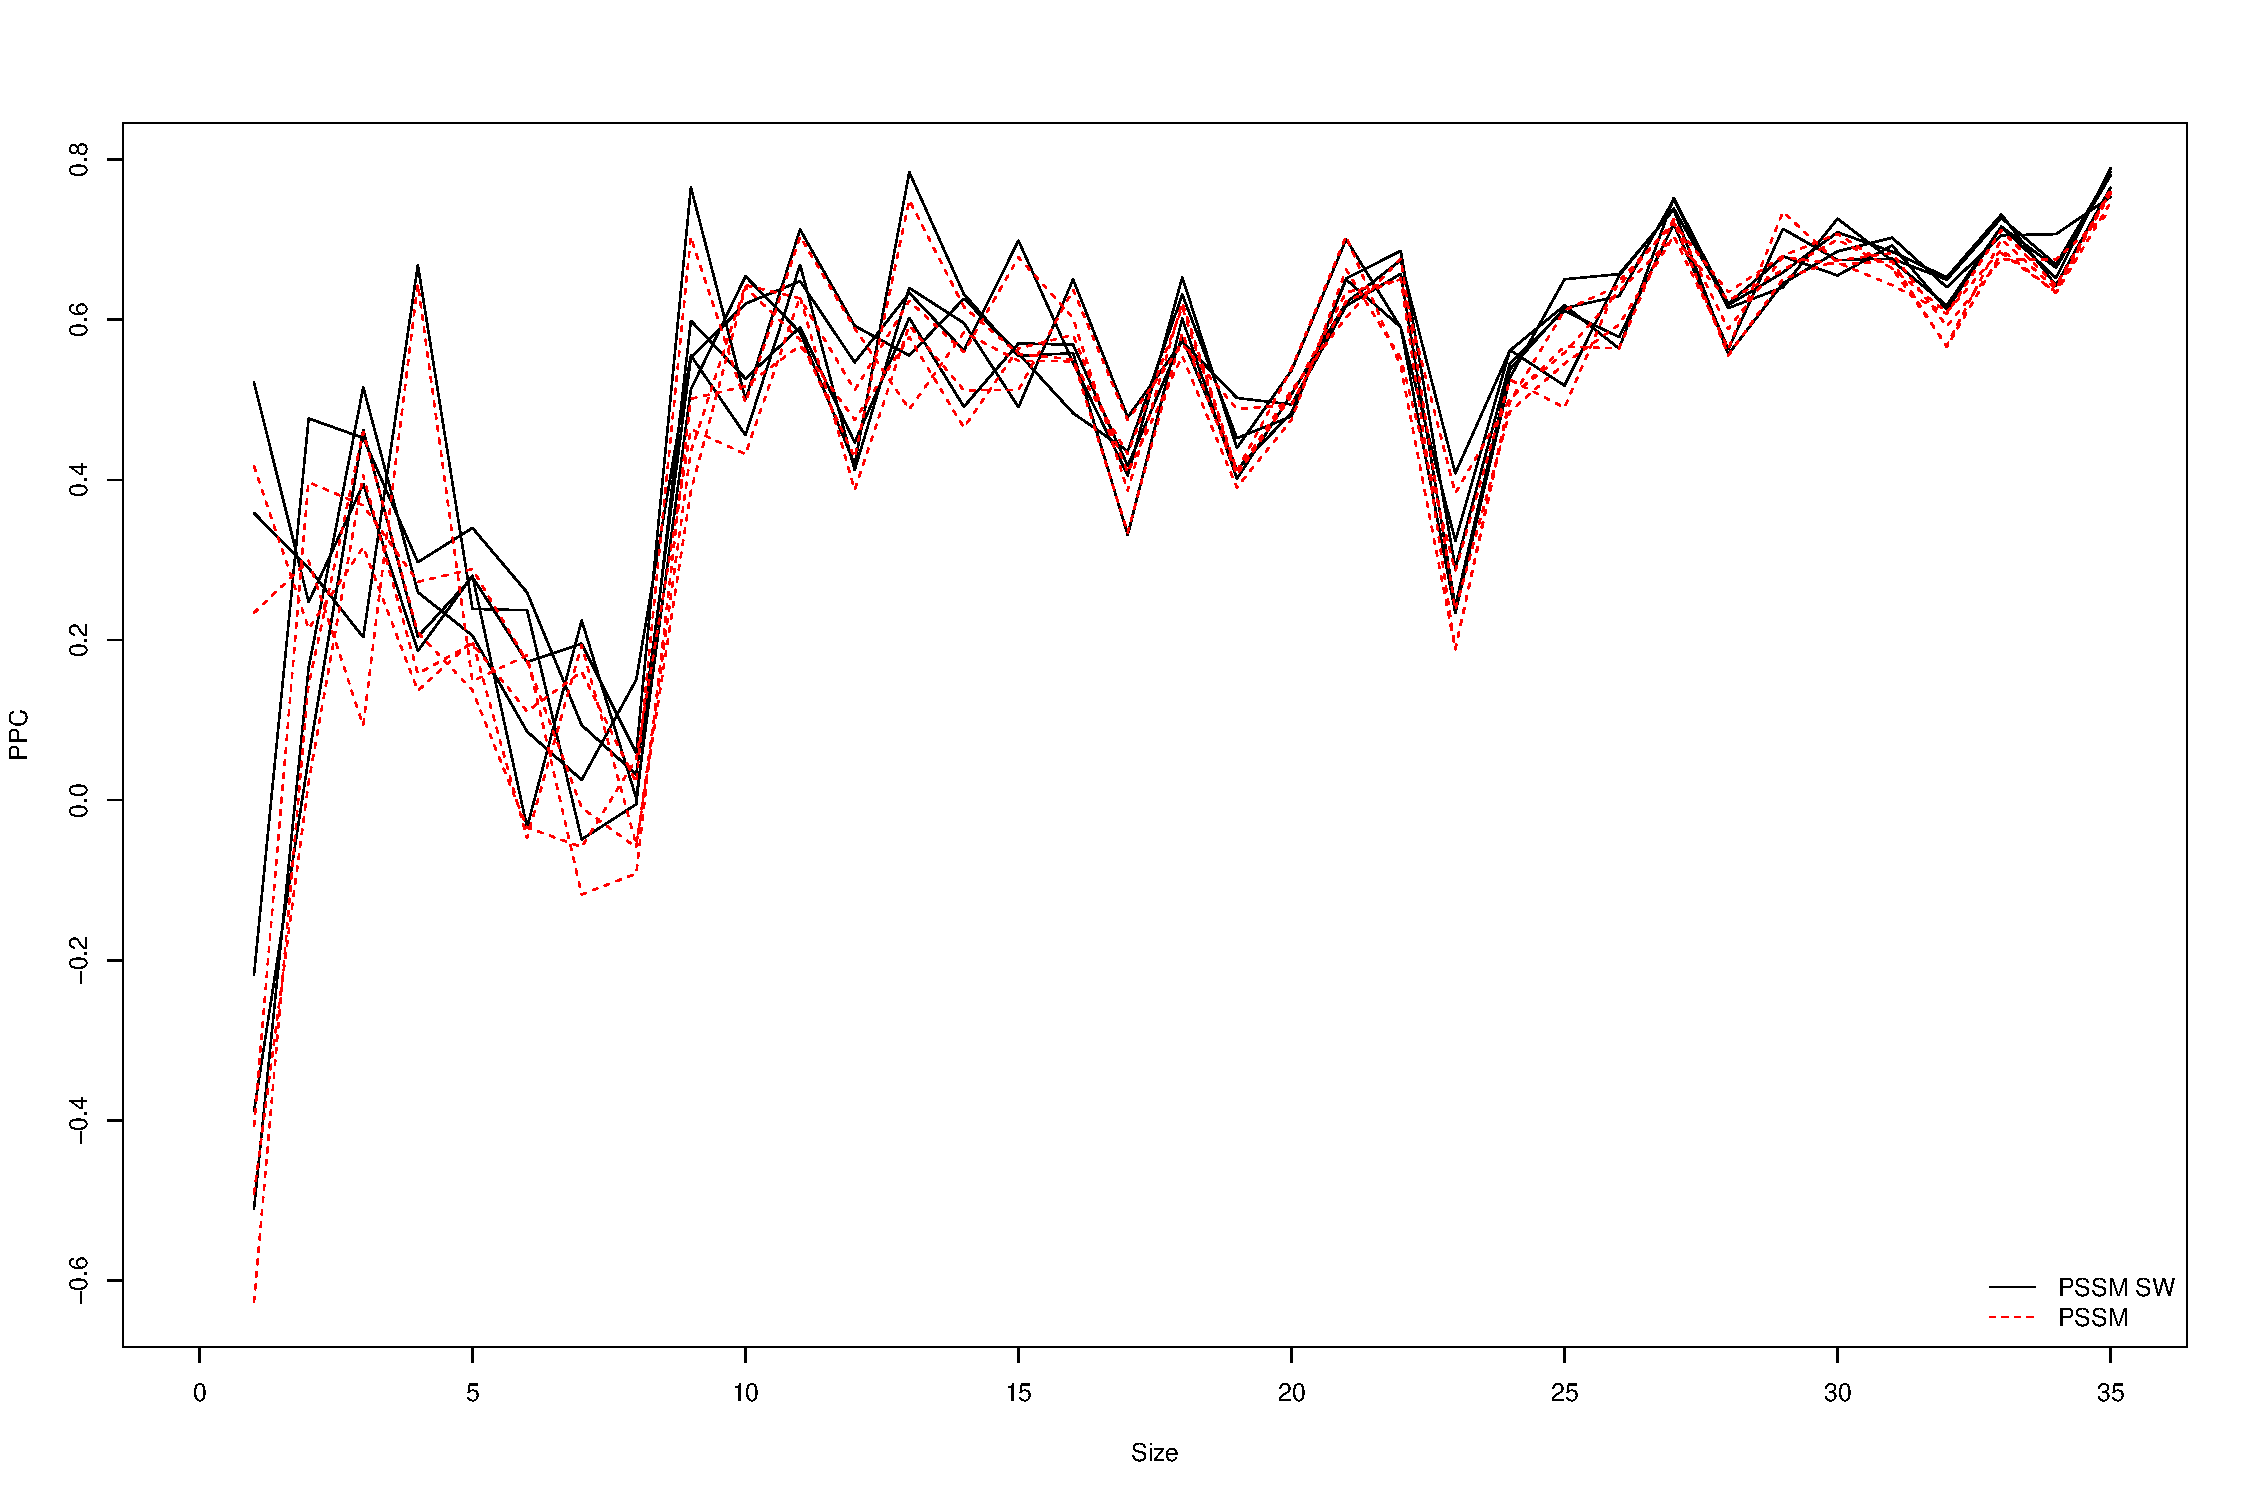
\includegraphics[width=18cm]{fig/pssmLN1.pdf}
\caption{Plot of the average Pearson Correlation Coefficent of the 5 test for the PSSM algorithm on each of the 35 alleles. The alleles are ordered by the number of binding peptide inside the data, the order is the following:
B5701, A3002, A2301, B4501, B1801, B4002, B4403, B4402, A2902, A2402, B5101, A2403, B5301, B5401, A3001, A2601, B0801, B3501, A6901, B2705, B1501, B5801, B4001, A6801, A3301, A0101, B0702, A6802, A0206, A0203, A0202, A3101, A1101, A0301 and A0201.}\label{fig:pssm1}
\end{center}
\end{figure*}

\begin{figure*}[ht]
\begin{center}
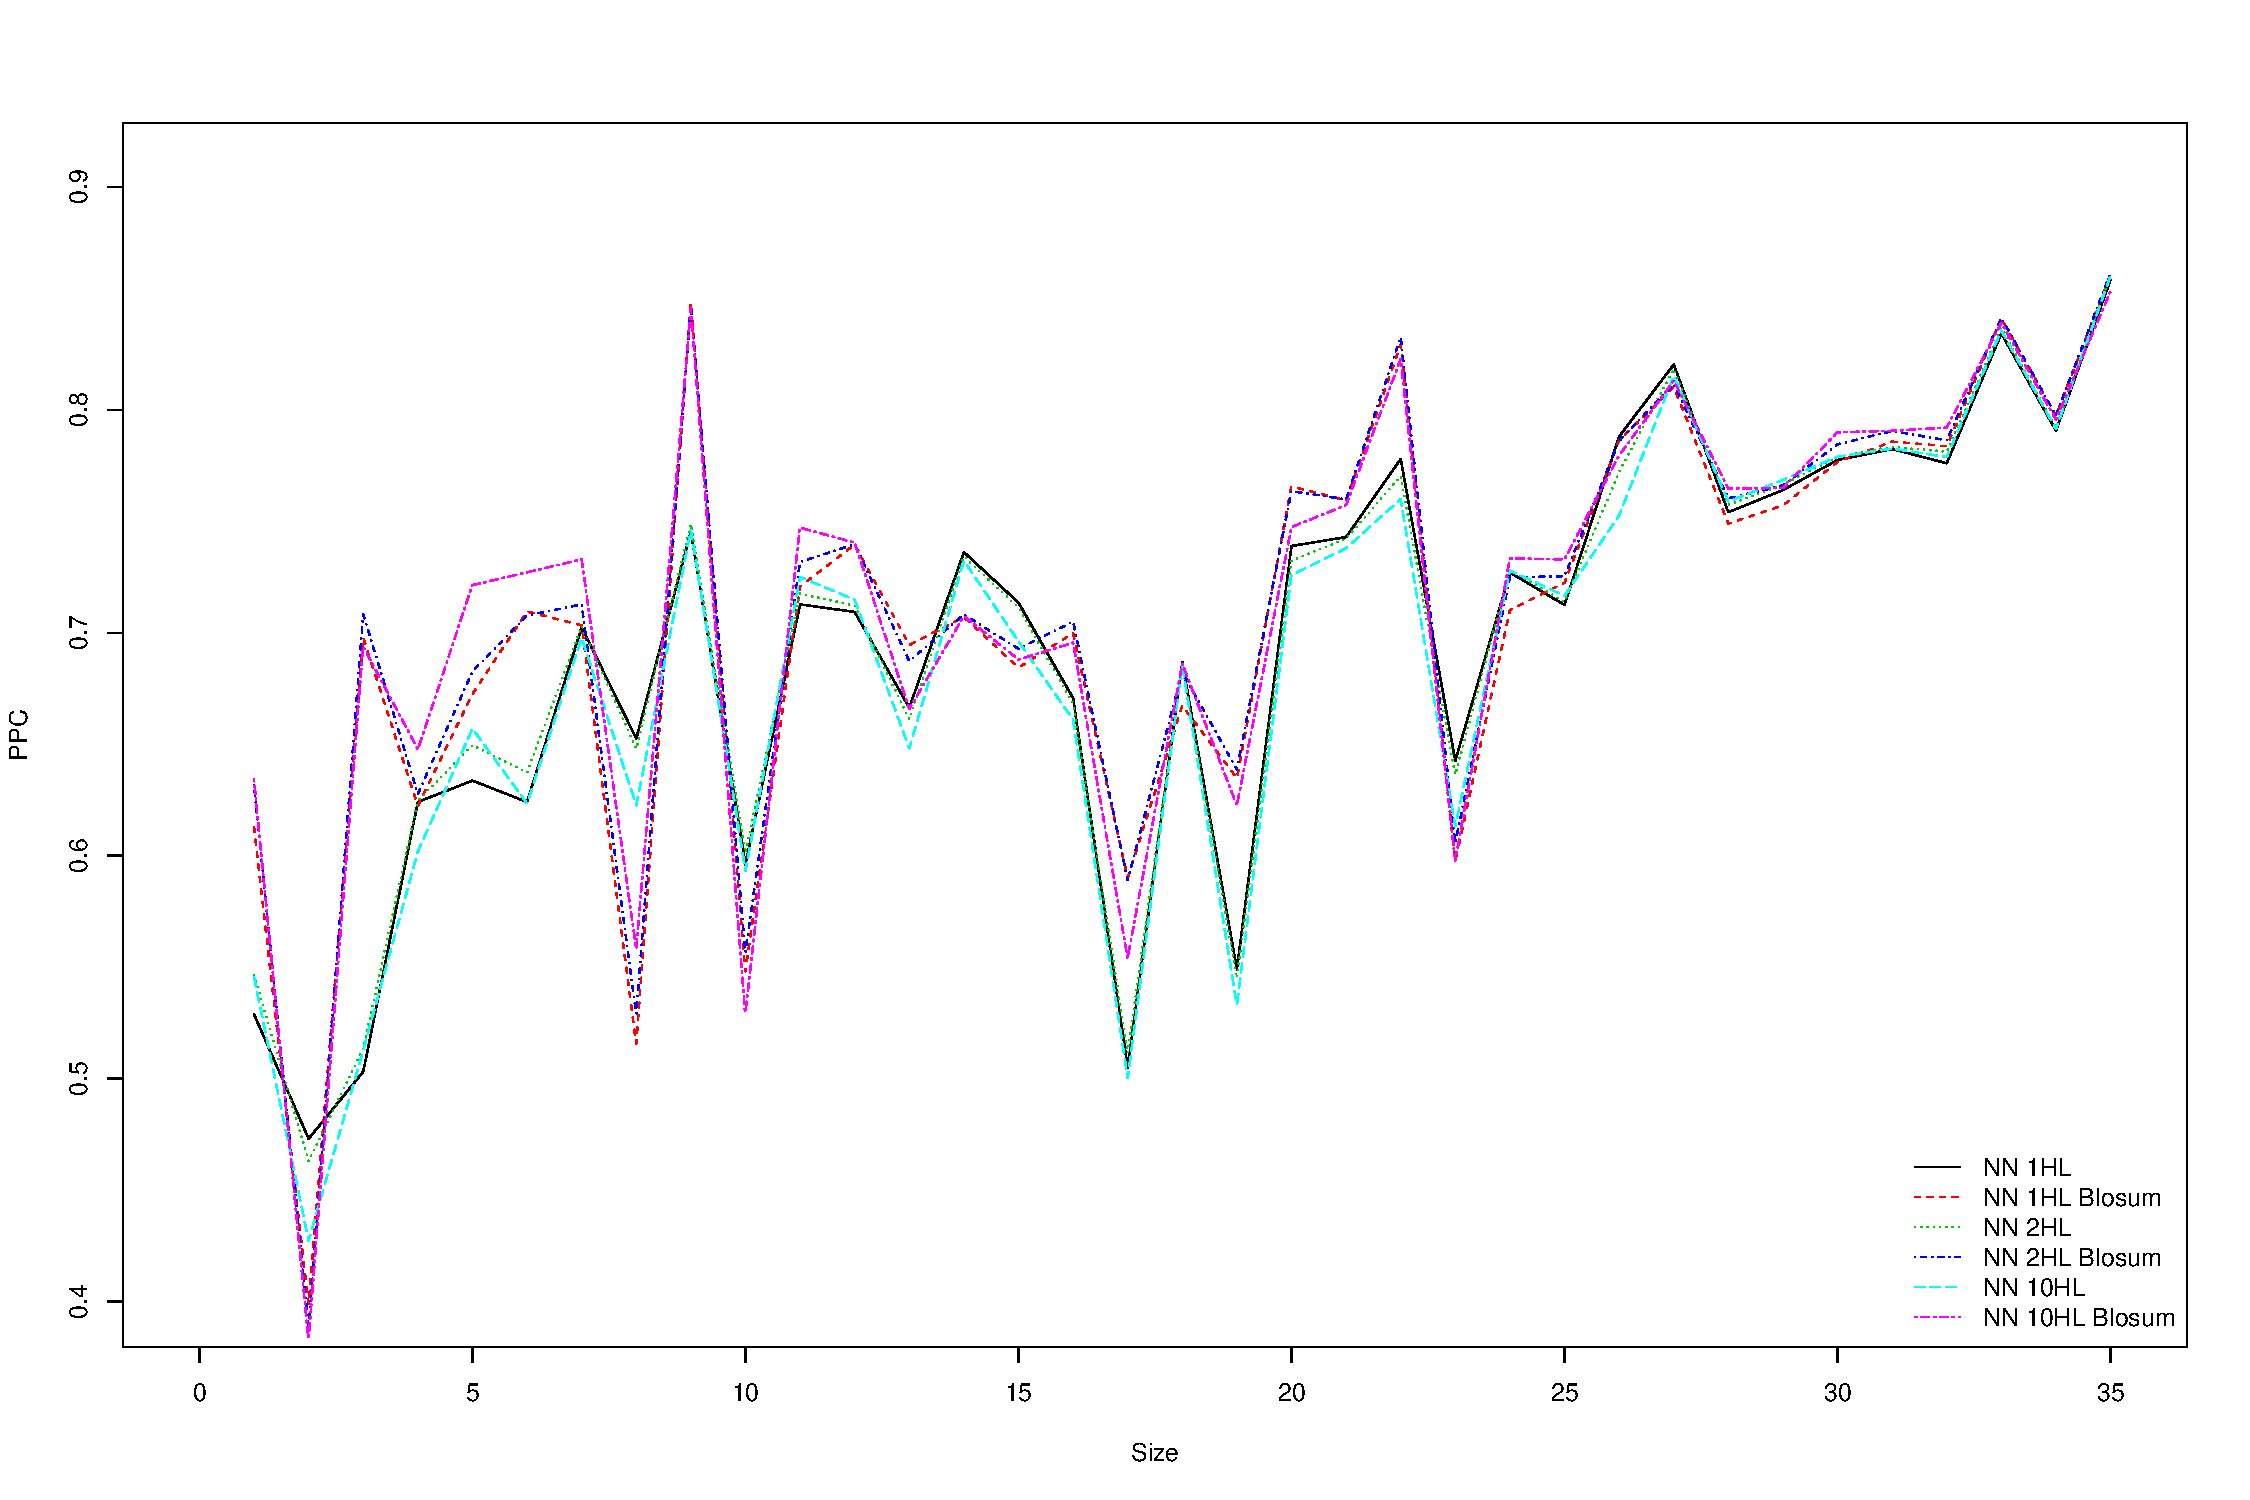
\includegraphics[width=18cm]{fig/annLNzoom.pdf}
\caption{Plot of the average Pearson Correlation Coefficent of the 5 test for the Artificial Neural Network algorithm on each of the 35 alleles. The alleles are ordered by the number of peptide in the dataset. The order is the following:
B5701, A3002, A2301, B4501, B1801, B4002, B4403, B4402, A2902, A2402, B5101, A2403, B5301, B5401, A3001, A2601, B0801, B3501, A6901, B2705, B1501, B5801, B4001, A6801, A3301, A0101, B0702, A6802, A0206, A0203, A0202, A3101, A1101, A0301 and A0201.}\label{fig:ann1}
\end{center}
\end{figure*}

\begin{figure*}[ht]
\begin{center}
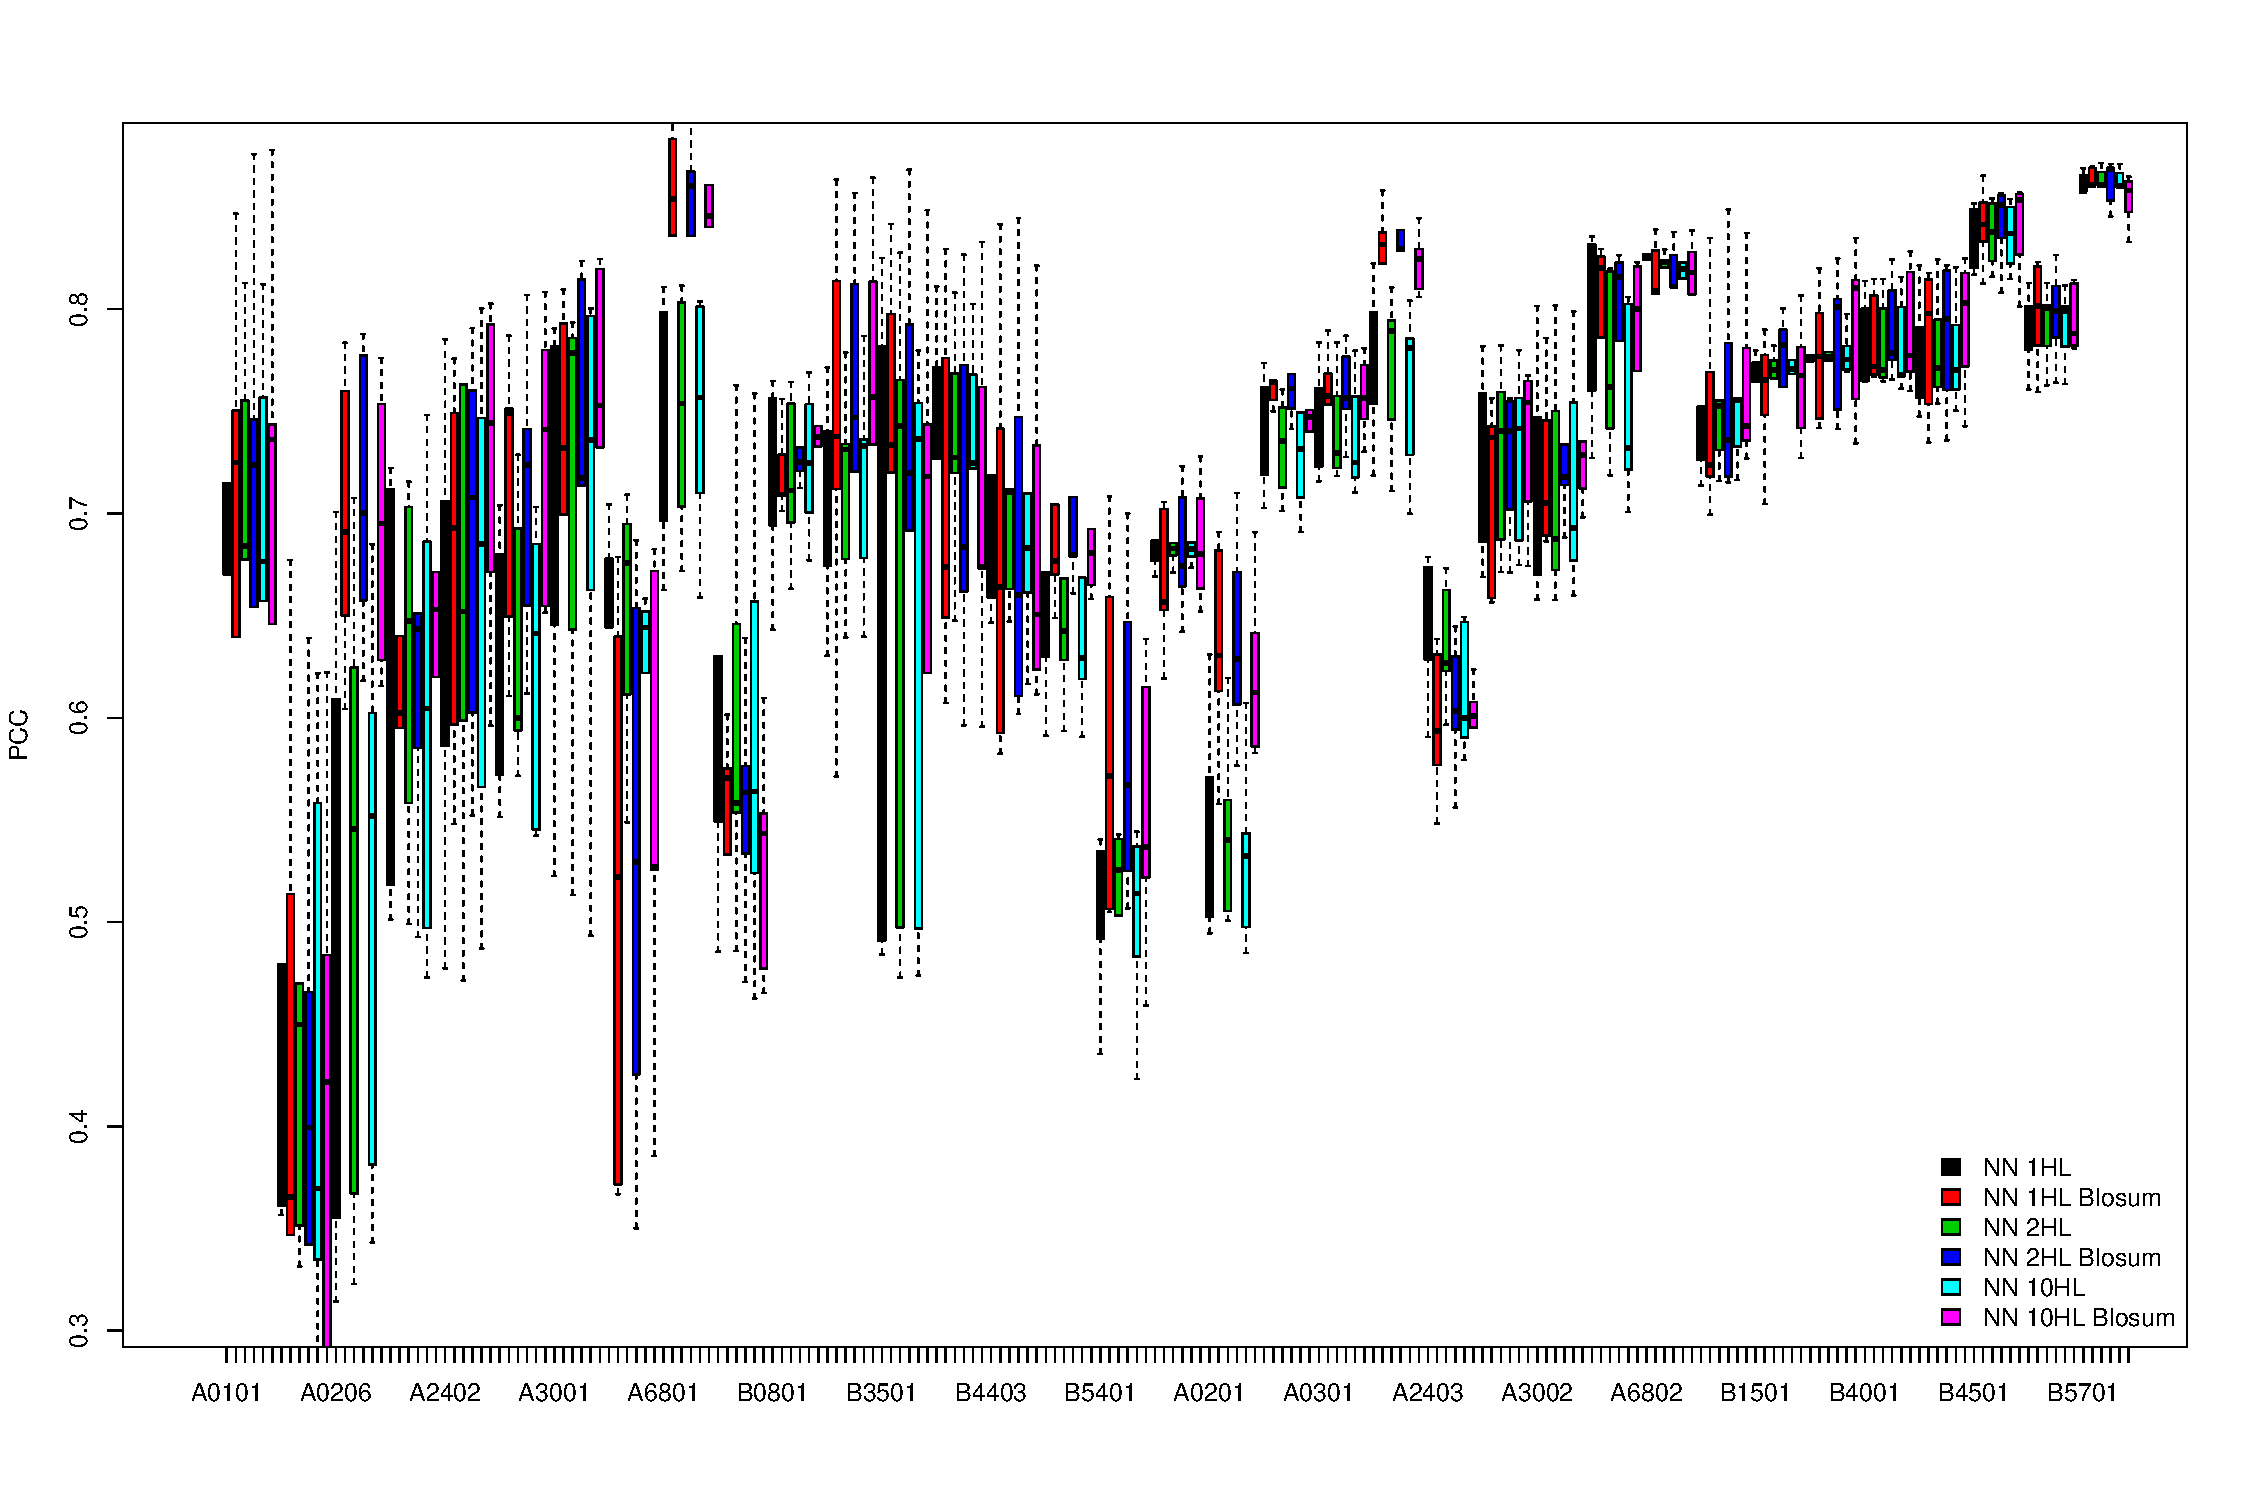
\includegraphics[width=18cm]{fig/annBX1.pdf}
\caption{Boxplot of the Pearson Correlation Coefficent of test with the ANN algorithm on the 35 different alleles. The alleles are ordered by the number of peptide in the dataset. The order in the y axis is the following:
B5701, A3002, A2301, B4501, B1801, B4002, B4403, B4402, A2902, A2402, B5101, A2403, B5301, B5401, A3001, A2601, B0801, B3501, A6901, B2705, B1501, B5801, B4001, A6801, A3301, A0101, B0702, A6802, A0206, A0203, A0202, A3101, A1101, A0301 and A0201.}\label{fig:ann2}
\end{center}
\end{figure*}
